\section{Complexity Considerations}
\label{sec:complexity}
% ================================================================================

In this section, we calculate upper bounds for the total number of test
executions to be performed when testing for failures refinement 
and---as a corollary---trace refinement.
Theorem~\ref{th:failurestest} specifies that all tests $U_F(j),\ 0\le j < pq$
need to be executed, where $p$ denotes the number of nodes in the transition
graph of the reference process $P$, and $q\ge p$ is an estimate for the
maximal number of nodes in the SUT's transition graph. Therefore, we will first
calculate a bound for the number of test executions to be performed for test
$U_F(j)$ and then summarise  these bounds over all $j$ from $0$ to $pq-1$.

For the worst-case estimate, we first introduce a CSP reference process $\pmax$
which 
turns out to be--given a fixed alphabet $\Sigma$---the test 
model leading to the maximal number 
of test executions for every $U_F(j)$ when considering large alphabets. In the case
of small alphabets and large values of $pq-1$, it will turn out below that a variant
of $\pmax$ will lead to the maximal number of executions. The conditions for this
can also be clearly specified.



%we assume that $P$ never allows for early
%deadlock (so $\minhits(P/s)$ is never empty) and that the SUT $Q$ is a
%correct failures refinement. Therefore, all test executions
%$(Q\parallel[\Sigma] U_F(j))$ stop after having run through a trace of $Q$ of
%length $j+1$, because their is no early termination due to entering branches
%(\ref{eq:ufa}), (\ref{eq:ufb}), or due to an illegal deadlock of $Q$. As can
%be seen from the specification of the test cases $U_F(j)$ (see
%Section~\ref{sec:finitecompletefails}), the number of executions ending in a
%$\epass$ event corresponds to the number $\ell$ of traces $s$ of $P$ with
%length equal to $j$, multiplied by the number $h$ of minimal hitting sets in
%$\minhits(P/s)$. For the tests $U_T(j)$ verifying trace refinement (see
%Section~\ref{sec:finitecomplete}), the number of executions equals $\ell$,
%since there is no equivalent in $U_T(j)$ to checking different hitting sets
%in the last step of a test execution. \fixme{But doesn't this add to the
%number of executions?} \fxnote{jp: should be clear now from the revised test}




% -------------------------------------------------------------------------
\subsection{A Reference Process With Maximal Test Complexity}


% -----------------------------------------------------------------------------
\subsubsection*{Process Definition and Basic Properties}
Given an alphabet $\Sigma$ of size $\card{\Sigma} = n\ge 2$, define
a collection of subsets of $\Sigma$ by
\begin{equation}\label{eq:defC}
{\cal C} = \{ A\subseteq\Sigma~|~\card{A} = n - \lfloor\frac{n}{2}\rfloor + 1 \}.
\end{equation}
%
With this choice of ${\cal C}$, define
\begin{equation}\label{eq:pmax}
\pmax = \Intchoice_{A\in{\cal C}} e:A\then \pmax
\end{equation}
%
The important properties of $\pmax$ are summarised in the following lemma.
%
\begin{lemma}\label{lemma:pmax}
Given alphabet $\Sigma$ with cardinality $\card{\Sigma} = n\ge 2$,
process $\pmax$ fulfils
%
\begin{eqnarray}
{}[\pmax/s]^0 & = & \Sigma \quad\text{for all $s\in \Sigma^*$}
\label{eq:pmaxa}
\\
\trc(\pmax) & = & \Sigma^*
\label{eq:pmaxb}
\\
\minaccs(P/s) & = & {\cal C} \quad\text{for all $s\in \Sigma^*$}
\label{eq:pmaxc}
\\
\minhits(P/s) & = & \minhits({\cal C}) \quad\text{for all $s\in \Sigma^*$}
\label{eq:pmaxe}
\\
\card{\minhits(P/s)} & = & \binom{n}{\lfloor\frac{n}{2}\rfloor} 
\quad \text{for all $s\in \Sigma^*$}
\label{eq:pmaxd}
\\
\minhits({\cal C})  & = & \{ H\subseteq \Sigma~|~\card{H} = \lfloor\frac{n}{2}\rfloor\}
\label{eq:pmaxf}
\end{eqnarray}
\end{lemma}
\begin{proof}
 Since  
$
\bigcup_{A\in{\cal C}} A = \Sigma
$
by construction of ${\cal C}$, $[\pmax]^0 = \Sigma$. Since $\pmax/e = \pmax$ for all
$e\in\Sigma$, this proves statements (\ref{eq:pmaxa}) and (\ref{eq:pmaxb}).
The internal choice construct used in the specification of $\pmax$ implies
$\minaccs(\pmax) = {\cal C}$. Again, $\pmax/e = \pmax$ for all
$e\in\Sigma$ implies $\minaccs(\pmax/s) = {\cal C}$ for all traces of $\pmax$, so this shows (\ref{eq:pmaxc}). Statement (\ref{eq:pmaxe}) is a direct consequence
of (\ref{eq:pmaxc}).

Let $H$ be any minimal hitting set of ${\cal C}$. Then
$H$ contains at least $\lfloor{\frac{n}{2}}\rfloor$ elements, because
otherwise $\card{\Sigma\setminus H} > n-\lfloor{\frac{n}{2}}\rfloor$, and any
subset $A\subseteq \Sigma\setminus H$ with cardinality
$n-\lfloor{\frac{n}{2}}\rfloor+1$  would be contained in ${\cal C}$, but satisfy
$A\cap H=\varnothing$. Since
$\lfloor{\frac{n}{2}}\rfloor+n-\lfloor{\frac{n}{2}}\rfloor+1=n+1$, we
conclude
 that any $\lfloor{\frac{n}{2}}\rfloor$-element subset of $\Sigma$
 intersects  every element of ${\cal C}$.  Therefore, every minimal hitting set of ${\cal C}$ has exactly $\lfloor{\frac{n}{2}}\rfloor$ elements; this shows (\ref{eq:pmaxf})
and $\card{\minhits({\cal C})} = \binom{n}{\lfloor{\frac{n}{2}}\rfloor}$. The latter 
shows  (\ref{eq:pmaxd}) and completes the proof.
\xbox
\end{proof}

% -----------------------------------------------------------------------------
\subsubsection*{Test Cases of $\pmax$}
The test cases $U_F(j)$ generated from $\pmax$ 
can never enter branch (\ref{eq:ufa}), because $\pmax/s$ has initials $\Sigma$ for
all traces $s\in\trc(\pmax)$ according to Lemma~\ref{lemma:pmax}, (\ref{eq:pmaxa}).
Moreover, they can never enter branch (\ref{eq:ufb}), because $\minhits(\pmax/s)$
is never empty according to Lemma~\ref{lemma:pmax}, (\ref{eq:pmaxd}).
Finally, the minimal hitting sets used to probe the SUT at the end of a
non-blocking  test execution are always the hitting sets of ${\cal C}$ 
according to Lemma~\ref{lemma:pmax}, (\ref{eq:pmaxe}).
This results in a test case structure
\begin{eqnarray*}
\label{eq:UFP}
U_F(j) & = & U_F(j,0,\ii n)
\\
U_F(j,k,n) & = &   (k < j) \& \big(e:\Sigma   \then U_F(j,k+1,t(n,e) \big)
\\ & & \extchoice  
\\ & & (k = j) \& \big( \Intchoice_{H\in\minhits({\cal C})} (e:H   \then \epass \then\Stop   )  \big)
\end{eqnarray*}



% -----------------------------------------------------------------------------
\subsubsection*{Maximal Number of Test Executions for $\pmax$}

When considering the number of test executions to be performed by 
$U_F(j)$ against some SUT $Q$ for all $j=0,\dots,pq-1$, the maximal number of 
test executions is only reached if $Q$ is a correct refinement of the reference
process or if it fails in the very last execution of the very last $U_F(j)$ 
executed against $Q$. If an erroneous behaviour of $Q$ is revealed before this
very last execution, the test suite is stopped and $Q$ is fixed before
executing the suite again.
Therefore, we consider only correct SUTs $Q$ when determining the
maximal number of executions that can be executed.

For the  $U_F(j)$ generated from $\pmax$, the number of test executions
 to be performed is maximal if $\pmax\lessdet_F Q$ and 
$\trc(Q) = \Sigma^*$. In such a situation, no test execution blocks early, because
$Q/s$ can always engage into some $e\in\Sigma$   while $\#s<j$ and will never block
in the last step when $\#s = j$ and a hitting set $H\in\minhits({\cal C})$ is 
offered by the test case. The resulting number of executions is
%
\begin{equation}
\label{eq:maxexec}
n^{j}\cdot \binom{n}{\lfloor\frac{n}{2}\rfloor},
\end{equation}
%
because all traces up to length $j$ can be executed with $U_F(j)$ entering branch
(\ref{eq:ufc}), and each of these traces is followed by one event
from each of the hitting sets of ${\cal C}$.

The number of executions specified in (\ref{eq:maxexec}) is indeed maximal for
all reference processes $P$ fulfilling $\minhits(P/s)\neq\varnothing$ for all
traces $s$. All these processes can never enter branch (\ref{eq:ufb}), and,
if an execution with an SUT entered branch (\ref{eq:ufa}), this would only lead to early termination of the whole test suite, because a failure has been detected.
As a consequence, $\card{\Sigma}^{j}$ is the maximal number of traces to be executed 
up to length $j$, and from Theorem~\ref{th:sperner} we know that the number
$\binom{n}{\lfloor\frac{n}{2}\rfloor}$ of hitting sets to be tested at the end of each trace of length $j$ is already maximal.

Summing up  formula 
(\ref{eq:maxexec}) over all test cases $U_F(0),\dots,U_F(pq-1)$ to be executed and applying the formula for the sum of a geometric progression,  this results in
%
\begin{equation}\label{eq:pmaxcomplexity}
\sum_{j=0}^{pq-1} n^{j}\cdot \binom{n}{\lfloor\frac{n}{2}\rfloor}  = 
\binom{n}{\lfloor\frac{n}{2}\rfloor}\cdot\frac{1-n^{pq}}{1-n}\quad\text{with $n=\card{\Sigma}$}
\end{equation}
%
as the maximal number of test executions to be performed when testing an error-free
SUT $Q$ against reference process $\pmax$. This maximum is met when $Q$ equals $\Sigma^*$.
 


% -----------------------------------------------------------------------------
\subsubsection*{Considering Empty Collections of Minimal Hitting Sets} 

The argument so far has shown that reference process $\pmax$ requires the most test 
executions among all CSP processes $P$ whose collections of minimal hitting sets  
$\minhits(P/s)$ are never empty for any trace $s$, so that the branch 
(\ref{eq:ufb}) of the related test cases $U_F(j)$ can never be entered.  
Lemma~\ref{lemma:failureshittingsets} implies that an empty collection 
$\minhits(P/s)$
is equivalent to $(s,A)\in\fails(P)$ for all $A\subseteq\Sigma$. This is equivalent to
$\maxrefs(P/s) = \{ \Sigma \}$ or $\minaccs(P/s) = \{ \varnothing\}$.

It remains to 
consider the question whether reference processes $Z$ possessing failures $(s,\Sigma)$
may require more test executions for their associated tests $U_F(j)$ than the bound
given for $\pmax$ in (\ref{eq:pmaxcomplexity}). To this end, we consider the following process $Z$ whose behaviour is quite close to that of $\pmax$ with the only difference
that after some pre-defined trace $\ol s \in\Sigma^*$ with $\#\ol s < pq$, 
the process has $\Stop$ as
an internal choice, so that $Z/s = \big(\Intchoice_{A\in{\cal C}} e:A\then \pmax\big) \intchoice \Stop$, and, consequently, $\minhits(Z/s) = \varnothing$.

In the following specification of $Z$, given traces $s_1,s_2\in\Sigma^*$, the Boolean 
expression $ s_1 < s_2$ evaluates to $\ist$ if and only if $s_1$ is a true prefix of $s_2$.
\begin{eqnarray*}
Z & = & Z_1(\varepsilon)
\\
Z_1(s) & = & (s < \ol s)\&\big( \Intchoice_{A\in{\cal C}} e:A\then Z_1(s.e)  \big)
\\ & & \extchoice
\\ & & (s \not< \ol s) \& \pmax
\\ & & \extchoice
\\ & & (s = \ol s) \& \big( \Intchoice_{A\in{\cal C}} e:A\then \max  \big)
\intchoice \Stop
\end{eqnarray*}
%
It is easy to see that $\trc(Z) = \trc(\pmax) =\Sigma^*$ and that for all 
traces $s\neq\ol s$, $\minhits(Z/s) = \minhits(P/s) = \minhits({\cal C})$ as specified
in Lemma~\ref{lemma:pmax}.

When comparing the test cases $U_F(j)$ generated from $\pmax$ and the test cases
$U_F^Z(j)$ created from $Z$, we note that
\begin{enumerate}
\item For $j < \#\ol s$, the test cases  $U_F(j)$ and $U_F^Z(j)$ are identical.
\item For $j = \#\ol s$, branch (\ref{eq:ufb}) can be entered by $U_F^Z(j)/\ol s$, while it is blocked for $U_F(j)/\ol s$, and branch (\ref{eq:ufd}) is blocked
for  $U_F^Z(j)/\ol s$, while it can be entered by $U_F(j)/\ol s$. As a consequence,
the maximal number of executions that can be performed by $U_F^Z(j)$ against the SUT 
is 
\begin{equation}
(n^{j} - 1)\cdot \binom{n}{\lfloor\frac{n}{2}\rfloor} + 1
\end{equation}
according to (\ref{eq:maxexec}): we win one additional execution by entering 
branch (\ref{eq:ufb}) after $\ol s$ and lose $\binom{n}{\lfloor\frac{n}{2}\rfloor}$ executions
by no longer being able to enter branch (\ref{eq:ufd}) after $\ol s$.

\item For $j > \#\ol s$, one execution is won by entering 
branch (\ref{eq:ufb}) after $\ol s$, no executions are lost.
\end{enumerate}
%
Summing up over $j = 0,\dots,pq-1$, this results in a difference of 
%
\begin{equation}
(pq  - \#\ol s) - \binom{n}{\lfloor\frac{n}{2}\rfloor}
\end{equation}
executions for the test cases $U_F^Z(j),\ j=0,\dots,pq-1$ in comparison to 
the test cases $U_F(j),\ j=0,\dots,pq-1$. To assess this formula, see the function
table for the first 19  arguments of $\binom{n}{\lfloor\frac{n}{2}\rfloor}$ shown
in Table~\ref{table:binom}.
%
\begin{table}[htp]
\caption{Function table of $\binom{n}{\lfloor\frac{n}{2}\rfloor}$ for arguments
$n = 2,\dots,20$.}
\begin{center}
\begin{tabular}{c||c|c|c|c|c|c|c|c|c|c|c|c|c|c|c|c|c|c|c}
$n$ & 2 & 3 & 4 & 5 & 6 & 7 & 8 & 9 & 10 & 11 & 12 & 13  & 14 & 15 & 16 & 17 & 18 & 19 & 20 \\\hline
$\binom{n}{\lfloor\frac{n}{2}\rfloor}$ &
     2 & 3 & 6& 10 & 20 & 35 & 70 & 126 & 252 &
     462&924&1716&3432&6435&12870&24310&48620&92378&184756
\end{tabular}
\end{center}
\label{table:binom}
\end{table}
%
The analysis above leads to the following complexity result.
%
\begin{theorem}
Given a process alphabet $\Sigma$ with cardinality $
\card{\Sigma} = n$, consider a fault model ${\cal F} = (P,\lessdet_F,{\cal D})$, such that
the normalised transition graph of $P$ has $p$ states, and the fault domain 
${\cal D}$ contains all processes $Q$ over alphabet $\Sigma$, such that $G(Q)$ has at most $q$ states. Then, if $pq < \binom{n}{\lfloor\frac{n}{2}\rfloor}$, the complete
test suite $\TS_F = \{ U_F(j)~|~0 \le j < pq  \}$ created from $P$ according to Theorem~\ref{th:failurestest}
requires at most 
%
\begin{equation*}
\binom{n}{\lfloor\frac{n}{2}\rfloor}\cdot\frac{1-n^{pq}}{1-n}
\end{equation*}
%
test executions.
\xbox
\end{theorem}


% -------------------------------------------------------------------------
\subsection{Estimation of $\ell$}
The first factor $\ell$ has worst-case upper bound $\ell\le \card{\Sigma}^j$.
As an example where this upper bound is really met, we consider the reference
process
\[
RUN(\Sigma) = e:\Sigma \then RUN(\Sigma).
\]
The normalised transition graph of this process has a single state, and its initials
are $[RUN(\Sigma)]^0 = \Sigma$. Therefore, the associated test process $U_F(j)$ can
never enter branches (\ref{eq:ufa}) and (\ref{eq:ufb}), but there are exactly
$\card{\Sigma}^j$ different traces of length $j$ exercising branch (\ref{eq:ufc})
for each of their events.

% -------------------------------------------------------------------------
\subsection{Estimation of $h$}
Given a set $\minaccs(P/s) = \{ A_1,\dots, A_\alpha \}$ of   minimal
acceptances, the cardinality   $h = \card{\minhits(P/s)}$ has the upper bound
\[
h \le \binom{n}{\lfloor\frac{n}{2}\rfloor}, \quad \text{where $n = \card{\Sigma}$.}
\]
This follows from Theorem~\ref{th:sperner}, since $\minhits(P/s)$ is a
Sperner Family~(see Section~\ref{sec:sperner}). The next theorem shows that
this upper bound can really be reached by collections of minimal hitting sets
associated with a CSP process state.

\begin{theorem}
\label{th:upperboundh}
Let  $\Sigma$  be an alphabet with cardinality $n\ge 2$.  Then
there exists a CSP process $P$ with
\[
\card{\text{minHit}(P)} = \binom{n}{\lfloor\frac{n}{2}\rfloor}.
\]
\end{theorem}
\begin{proof}
Let ${\cal C}$ be the collection of all subsets of $\Sigma$ with cardinality
$n-\lfloor{\frac{n}{2}}\rfloor+1$. Then the CSP process
\[
P = \Intchoice_{A\in {\cal C}} e:A\then P
\]
fulfils $\minaccs(P) = {\cal C}$. Let $H$ be any minimal hitting set of ${\cal C}$. Then
$H$ contains at least $\lfloor{\frac{n}{2}}\rfloor$ elements, because
otherwise $\card{\Sigma\setminus H} > n-\lfloor{\frac{n}{2}}\rfloor$, and any
subset $A\subseteq \Sigma\setminus H$ with cardinality
$n-\lfloor{\frac{n}{2}}\rfloor+1$  would be contained in ${\cal C}$, but satisfy
$A\cap H=\varnothing$. Since
$\lfloor{\frac{n}{2}}\rfloor+n-\lfloor{\frac{n}{2}}\rfloor+1=n+1$, we
conclude
 that any $\lfloor{\frac{n}{2}}\rfloor$-element subset of $\Sigma$
 intersects  every element of ${\cal C}$.  Therefore, every minimal hitting set of ${\cal C}$ has exactly $\lfloor{\frac{n}{2}}\rfloor$ elements,
so $\card{\minhits({\cal C})} = \binom{n}{\lfloor{\frac{n}{2}}\rfloor}$.
\xbox
\end{proof}
%
To get an approximation of the maximal size of $\minhits(P/s)$ for large $n$,
recall Stirling's approximation~\cite[p.~112]{Graham:1994:CMF:562056}
\[
m! \approx \sqrt{2\pi m} \cdot \big( \frac{m}{e} \big)^m, \quad\text{where $e$ denotes the Euler Number.}
\]
Applying this approximation when $n = \card{\Sigma}$ is even and $m = (n/2)$
results in
\[
h \le \binom{2m}{m} \approx \frac{4^m}{\sqrt{\pi m}} =
\frac{2^\card{\Sigma}}{\sqrt{2\pi \card{\Sigma}}}.
\]
%
We note that, due to this approximation result,
$h$ is   smaller than $2^{\card{\Sigma}}-1$, the cardinality of the
non-empty subsets of $\Sigma$.

\begin{theorem}\label{th:numexecP}
Let $U_F(j)$ be a test case derived from the 
process $P$ specified in the proof of Theorem~\ref{th:upperboundh}. Then
$U_F(j)$ has
\[
\binom{n}{\lfloor\frac{n}{2}\rfloor}\cdot \card{\Sigma}^j
\]
executions.
\end{theorem}
\begin{proof}
Since the union of all minimal acceptances of $P$ equals $\Sigma$, 
the initials of $P$ satisfy $[P]^0 = \Sigma$. By construction, $P/e = P$
for any $e\in\Sigma$, so $\trc(P) = \Sigma^*$ and $[P/s]^0 = \Sigma$
for all $s\in\Sigma^*$. As a consequence, $U_F(j)$
may execute $\card{\Sigma}^j$ different traces, each time executing branch (\ref{eq:ufc}),
before finally entering branch (\ref{eq:ufd}). As shown in Theorem~\ref{th:upperboundh},
$\card{\minhits(P/s)} =  \binom{n}{\lfloor\frac{n}{2}\rfloor}$, so there are
$\binom{n}{\lfloor\frac{n}{2}\rfloor}$ possible executions of branch (\ref{eq:ufd})
after every trace of length $j$. This proves the theorem.
\xbox
\end{proof}

% -------------------------------------------------------------------------
\subsection{Upper Bounds of Test Executions for Checking Failures Refinement}

By Theorem~\ref{th:failurestest}, we need to execute the tests $U_F(j)$ for
$j = 0,\dots,(pq-1)$; this results in a worst-case bound defined below, where
we use the formula for the sum of the geometric progression.
%
\[
h\cdot \big( \frac{1-\card{\Sigma}^{pq}}{1-\card{\Sigma}} \big),\
 \text{or, asymptotically,}\  O(\frac{2^\card{\Sigma}}{\sqrt{2\pi \card{\Sigma}}}\cdot\card{\Sigma}^{(pq-1)}).
 \]
%
From Theorem~\ref{th:upperboundh} we know that the worst-case bound for $h$
above cannot be further reduced, since the full collection of minimal hitting
sets needs to be checked at the end of each execution of $U_F(j)$.

In~\cite{Hennessy:1988:ATP:50497}, it is suggested to test {\it every}
non-empty subset of $\Sigma$ whose events cannot be completely refused in a
given process state of the reference model; this leads to a worst-case
estimate of $2^{\card{\Sigma}}-1$ for the number of different sets to be
offered to the SUT in the last step of the test execution, so our approach
reduces the number of test executions in comparison
to~\cite{Hennessy:1988:ATP:50497} by a factor of $1/{\sqrt{2\pi
\card{\Sigma}}}$. In Fig.~\ref{fig:minhita}, the reduction is visualised by a
function plot of $2^{\card{\Sigma}}$ versus
$\frac{2^\card{\Sigma}}{\sqrt{2\pi \card{\Sigma}}}$.

In~\cite{DBLP:conf/icfem/CavalcantiG07}, the authors also use minimal hitting
sets\footnote{However, they are denoted by {\it minimal acceptances}
in~\cite{DBLP:conf/icfem/CavalcantiG07}.}, but they do not give an upper
bound for the number of test executions to be performed.

% .....................................................................................
 \begin{figure}
 %%\hspace*{-40mm}
 \begin{center}
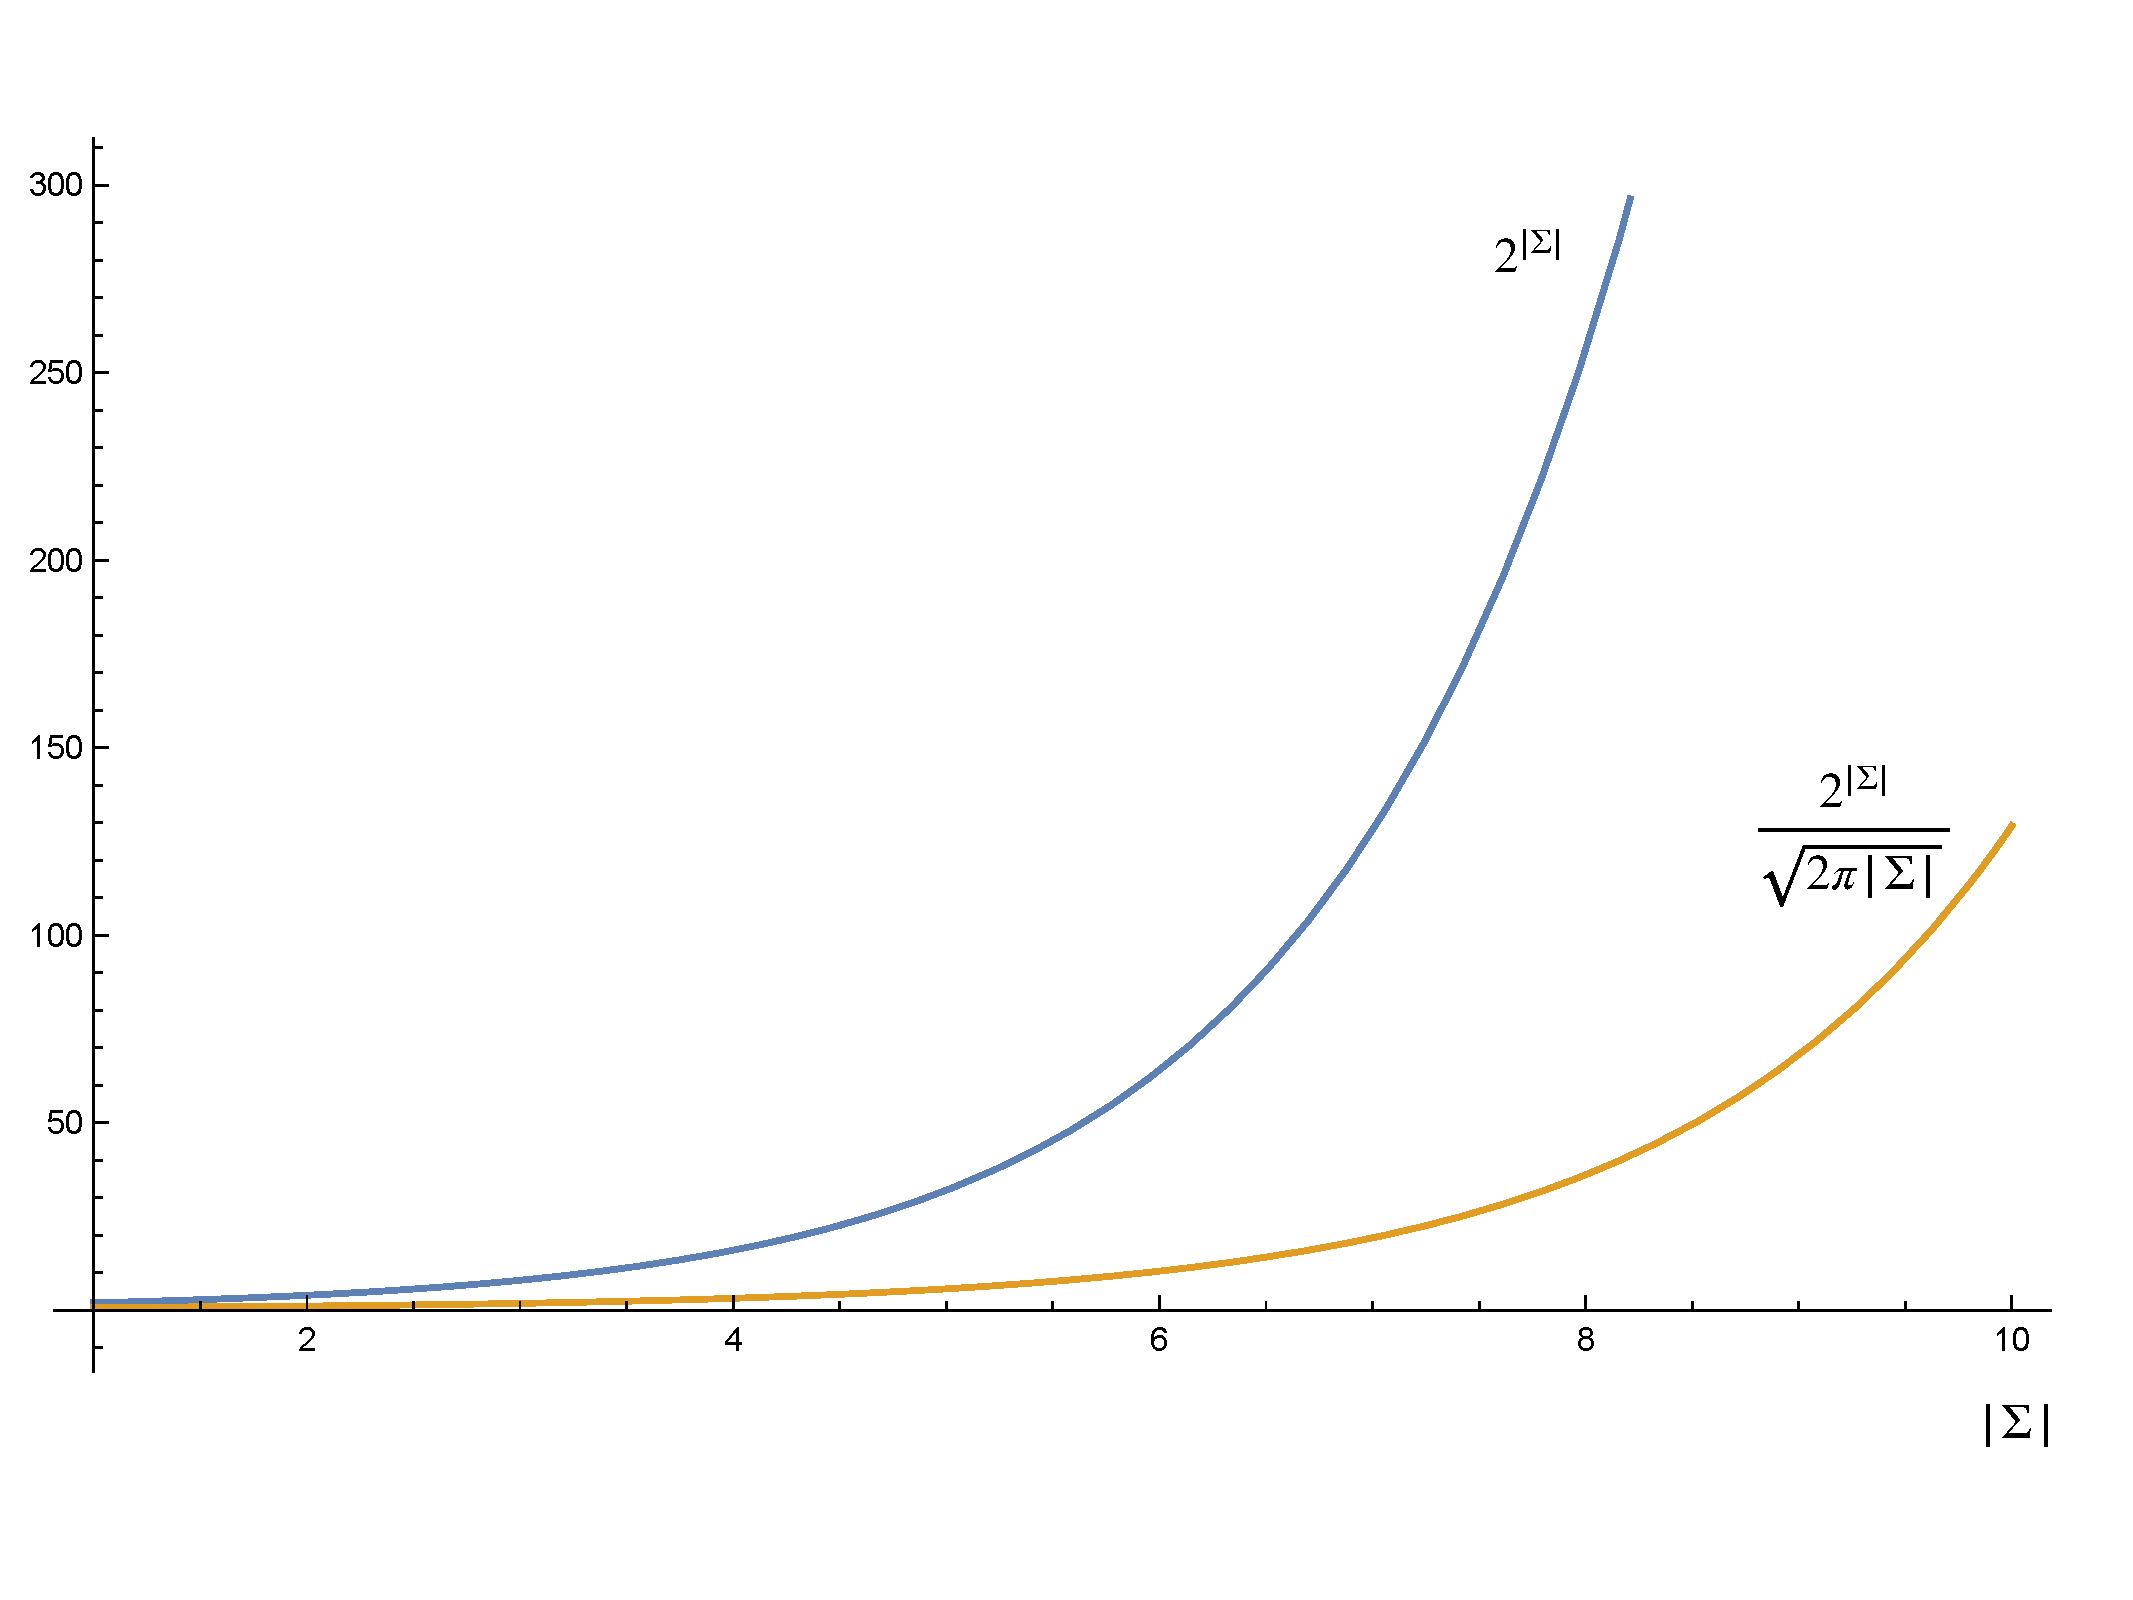
\includegraphics[width=.8\textwidth]{minhit-fig.pdf}
\end{center}
\vspace*{-10mm}
\caption{Function plot $2^{\card{\Sigma}}$ versus $\frac{2^\card{\Sigma}}{\sqrt{2\pi \card{\Sigma}}}$.}
 \label{fig:minhita}
 \end{figure}
% .......................................................................................

% -------------------------------------------------------------------------
\subsection{Upper Bounds of Test Executions for Checking Trace Refinement}

According to Theorem~\ref{th:tracetest}, a complete test suite checking trace
refinement just contains the adaptive test case $U_T(pq-1)$. As derived for
$U_F(j)$ above, the number of executions performed by $(Q\parallel[\Sigma]
U_T(pq-1))$ is bounded by $\card{\Sigma}^{pq-1}$.

% -------------------------------------------------------------------------
\subsection{Upper Bound $pq$ for the Maximal Length of Test Traces}

According to Theorem~\ref{th:failurestest}, the tests $U_F(j)$ need to be
executed for $j = 0,\dots,pq-1$ to guarantee completeness.
 This means that the SUT is verified with test
traces up to, and including, length $pq$: recall from the test specification,
branch (\ref{eq:ufa}), that $U_F(j)$ will accept all traces $s.e$ with
$s\in\trc(P), \#s = j, e\not\in\trc(P/s)$, so erroneous traces up to length
$j+1$ are detected.

It is interesting to investigate whether this maximal length is really
necessary, or whether one could elaborate alternative complete test
strategies where the SUT is tested with shorter traces only. Indeed, an
example  presented in~\cite[Exercise~5]{PeleskaHuangLectureNotesMBT} shows
that when testing for equivalence of deterministic FSMs, it is sufficient to
test the SUT with traces of significantly shorter length.

The following example, however, shows that the maximal length $pq$ is really
required when testing for refinement.
%\begin{example}\label{ex:pq}
%Consider the CSP reference process $P$ and an erroneous implementation $Q$
%specified as follows.
%
%\begin{center}
%\begin{minipage}{.4\textwidth}
%\begin{eqnarray*}
%P & = & a \then P_1 \intchoice b \then P_1 \intchoice c \then P_1
%\\
%P_1 & = & a \then P \extchoice b\then P
%\end{eqnarray*}
%\end{minipage}
%\hfill
%\begin{minipage}{.4\textwidth}
%\begin{eqnarray*}
%Q & = & a\then Q_1 \extchoice b\then Q_1
%\\
%Q_1 & = & a\then Q_2 \extchoice b\then Q_2
%\\
%Q_2 & = & a\then Q \intchoice b\then Q
%\end{eqnarray*}
%\end{minipage}
%\end{center}
%
%
%\medskip
%Obviously, $P$'s normalised transition graph has 2 nodes, while $Q$'s graph
%has 3. It is easy to see (and can be checked with FDR4) that $P\lessdet_T Q$,
%but $\neg(P\lessdet_F Q)$. Furthermore, it can also be shown using FDR4 that
%the ``test passed condition''
%\[
%(\epass\then\Stop) \lessdet_F (Q\parallel[\Sigma] U_F(j))\hide \Sigma
%\]
%holds for $U_F(0),\dots,U_F(4)$, but fails for $U_F(5)$. So, the
%non-conformance of $Q$ cannot be detected by any test trace of length less or
%equal to 5, but is revealed (as expected from Theorem~\ref{th:failurestest})
%by a trace of length 6, because the last event offered by the test $U_F(5)$
%is refused by $Q$. \xbox
%\end{example}

\begin{figure}[htbp]
\begin{center}
\begin{minipage}{.4\textwidth}
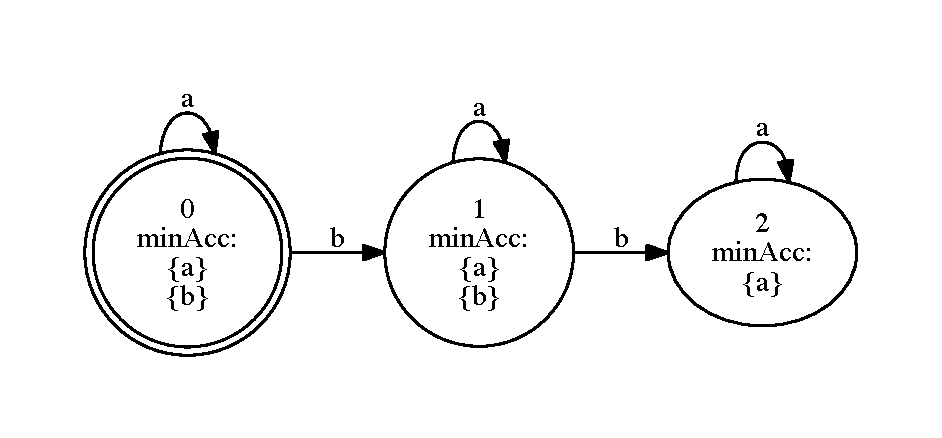
\includegraphics[width=1.2\textwidth]{theorem5p.pdf}
\end{minipage}
\hfill
\begin{minipage}{.55\textwidth}
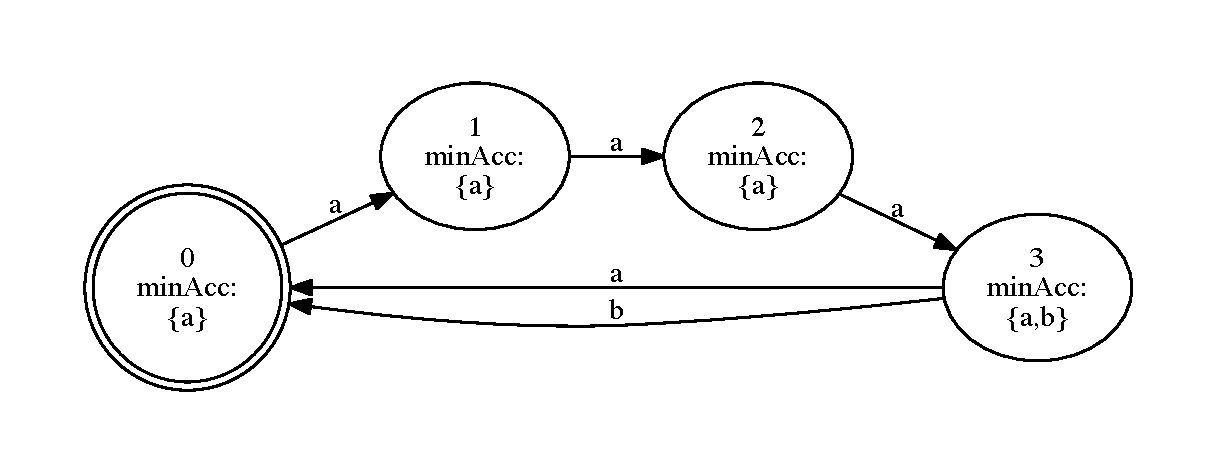
\includegraphics[width=1.2\textwidth]{theorem5q.pdf}
\end{minipage}
\caption{Transition graphs of $P$ (left) and $Q$ (right) from Example~\ref{ex:pq}
 for $p=3$ and $q=4$.}
\label{fig:examplepq}
\end{center}
\end{figure}

\begin{example}\label{ex:pq}
Consider the CSP reference process $P$ and an erroneous implementation $Q$
specified as follows.
%
\begin{eqnarray*}
P & = &  P(0)
\\
P(k) & = & (k < p-1) \& \big( (a \then P(k)) \intchoice ( b \then P(k+1))\big)
\\ & & \extchoice
\\ & & (k = p-1) \& (a \then P(k))
\\
Q & = & Q(0)
\\
Q(k) & = & (k < q-1) \& \big( a \then Q(k+1)    \big)
\\ & & \extchoice
\\ & & ( k = q-1)\& \big( a\then Q(0) \extchoice b\then Q(0)  \big)
\end{eqnarray*}
%
The normalised transition graphs of $P$ and $Q$ are depicted in
Fig.~\ref{fig:examplepq} for the case $p=3,\ q=4$. Using FDR4, it can be
shown for concrete values of $p$ and $q$ that the  ``test passed conditions''
\[
(\epass\then\Stop) \lessdet_F (Q\parallel[\Sigma] U_F(j))\hide \Sigma
\]
and
\[
(\epass\then\Stop) \lessdet_T (Q\parallel[\Sigma] U_T(j))\hide \Sigma
\]
hold for $j = 0,\dots,pq-2$. This means that none of the test cases $U_F(j)$
and $U_T(j)$ are capable of detecting failures and trace refinement
violations, if they only check traces up to length $pq-1$
(recall that this corresponds to $j\le pq-2$).

Process $Q$, however, neither conforms to $P$ in the failures refinement
relation, nor in the trace
refinement relation. This can only be seen when executing the test $U_F(pq-1)$ and
$U_T(pq-1)$, respectively. These tests fail, so this shows that $P\not\lessdet_F Q$ and
$P\not\lessdet_T Q$ according to Theorem~\ref{th:failurestest} and Theorem~\ref{th:tracetest}. Moreover, this shows that
the maximal trace
length $pq$ to be investigated in the tests cannot be further reduced without losing
the completeness property of the test suites.
\xbox
\end{example}
%
Generalising Example~\ref{ex:pq}, it can be shown that for any pair
$2\le p,q \in\mathbb{N}$,
there exist reference processes $P$ with $p$ states
and implementation processes $Q$ with $q$ states, such that
a violation of the trace refinement property
can only be detected with a trace of length $pq$. This is proven in the following
theorem. In the proof, we use the processes $P$ and $Q$ introduced in Example~\ref{ex:pq}.

% ----------------------------------------------------------------------------
\begin{theorem}\label{th:maxtracelen}
Let $2\le p,q \in\mathbb{N}$. Then there exists a reference process $P$ and an
implementation process $Q$ with the following properties.
\begin{enumerate}
\item $G(P)$ has $p$ states.
\item $G(Q)$ has $q$ states.
\item $P\not\lessdet_T Q$, and therefore, also $P\not\lessdet_F Q$.
\item $\forall s\in\trc(Q): \#s < pq\implies s\in\trc(P)$.
\item $Q\ conf\ P$.
\end{enumerate}
As a consequence, the upper bound $pq$ for the length of traces to be tested when checking for failures refinement or trace refinement
cannot be reduced without losing the test suite's completeness property.
\end{theorem}
% ----------------------------------------------------------------------------
\begin{proof}
Given $2\le p,q \in\mathbb{N}$, define reference process $P$ and implementation process $Q$ as in Example~\ref{ex:pq}. It is trivial to see that
$G(P)$ has $p$ nodes and $G(Q)$ has $q$ nodes, so statements 1 and 2 of the theorem hold.

Using regular expression notation, the traces of $P$ can be specified as
\[
\trc(P) = \prefs\big(  (a^*b)^{p-1}a^* \big),
\]
where $\prefs(M)$ denotes the set of all prefixes of traces in $M\subseteq\Sigma^*$,
including the traces of $M$ themselves.
The traces of $Q$ can be specified by
\[
\trc(Q) = \prefs\big( (a^{q-1}(a|b))^*  \big).
\]
It is easy to see that $\trc(Q)\not\subseteq\trc(P)$; for example, the trace
$(a^{q-1}b)^p$ is in $\trc(Q)\setminus\trc(P)$, because $P$-traces may contain at most $p-1$ $b$-events. This proves statement~3 of the theorem.

Let $s \in\trc(Q)$ be any trace of length $\#s = pq-1$. Then $s$ can be represented
by $s = (a^{q-1}(a|b))^{p-1}a^{q-1} \in \prefs\big( (a^{q-1}(a|b))^*  \big)$.
Then $s$ is also an element of $\trc(P)$, because $(a^{q-1}(a|b))^{p-1}a^{q-1}$
is also contained in $\prefs\big(  (a^*b)^{p-1}a^* \big)$: this is easy to see, since
$\prefs\big(  (a^*b)^{p-1}a^* \big)$ contains all finite sequences of $a$-events,
where at most $p-1$ events $b$ have been inserted. This proves statement 4 of the theorem.

To prove statement~5, we observe that the specification of $P$ implies (the
expression $(s\cnt b)$ denotes the number of $b$-events occurring in trace $s$)
\[
\minaccs(P/s) = \left\{
\begin{array}{ll}
\{ \{a\}, \{b\} \} & \text{for all $s\in\trc(P)$ with $(s\cnt b) <p-1$.}
\\
\{ \{a\} \} & \text{for all $s\in\trc(P)$ with $(s\cnt b) = p-1$.}
\end{array}
\right.
\]
and
\[
\minaccs(Q/s) = \left\{
\begin{array}{ll}
\{ \{a\}  \} & \text{for all $s\in\trc(Q)$ with $\#s \neq 0\mod(q-1)$.}
\\
\{ \{a,b\} \} & \text{for all $s\in\trc(P)$ with $\#s = 0\mod(q-1)$.}
\end{array}
\right.
\]
As a  consequence, the minimal acceptance set $A_P = \{a\}$ which is
contained in every $\minaccs(P/s)$ fulfils $A_P \subseteq A_Q$ for
any $A_Q\in\minaccs(Q/s)$, when $s\in\trc(P)\cap \trc(Q)$. Now Lemma~\ref{lemma:tgtrcref},
(\ref{eq:failrefb}) can be applied to conclude that $Q\ conf\ P$.
\xbox
\end{proof}
%
Since Theorem~\ref{th:maxtracelen} just states that a violation of trace
refinement may remain undetected if only traces shorter than $pq$ are checked
during tests, it can also be applied to our trace refinement tests.
Therefore, test suites $\{ U_T(j) \}$ with $j<pq-1$ are not complete. It is
discussed in Section~\ref{sec:conc} how the number of test traces to be
executed by complete test suites for failures or trace refinement can still
be reduced {\it without} reducing the maximal length.

% =================================================================================
